% Options for packages loaded elsewhere
% Options for packages loaded elsewhere
\PassOptionsToPackage{unicode}{hyperref}
\PassOptionsToPackage{hyphens}{url}
%
\documentclass[
  ignorenonframetext,
  aspectratio=169,
]{beamer}
\newif\ifbibliography
\usepackage{pgfpages}
\setbeamertemplate{caption}[numbered]
\setbeamertemplate{caption label separator}{: }
\setbeamercolor{caption name}{fg=normal text.fg}
\beamertemplatenavigationsymbolsempty
% remove section numbering
\setbeamertemplate{part page}{
  \centering
  \begin{beamercolorbox}[sep=16pt,center]{part title}
    \usebeamerfont{part title}\insertpart\par
  \end{beamercolorbox}
}
\setbeamertemplate{section page}{
  \centering
  \begin{beamercolorbox}[sep=12pt,center]{section title}
    \usebeamerfont{section title}\insertsection\par
  \end{beamercolorbox}
}
\setbeamertemplate{subsection page}{
  \centering
  \begin{beamercolorbox}[sep=8pt,center]{subsection title}
    \usebeamerfont{subsection title}\insertsubsection\par
  \end{beamercolorbox}
}
% Prevent slide breaks in the middle of a paragraph
\widowpenalties 1 10000
\raggedbottom
\usepackage{iftex}
\ifPDFTeX
  \usepackage[T1]{fontenc}
  \usepackage[utf8]{inputenc}
  \usepackage{textcomp} % provide euro and other symbols
\else % if luatex or xetex
  \usepackage{unicode-math} % this also loads fontspec
  \defaultfontfeatures{Scale=MatchLowercase}
  \defaultfontfeatures[\rmfamily]{Ligatures=TeX,Scale=1}
\fi
\usepackage{lmodern}

\ifPDFTeX\else
  % xetex/luatex font selection
\fi
% Use upquote if available, for straight quotes in verbatim environments
\IfFileExists{upquote.sty}{\usepackage{upquote}}{}
\IfFileExists{microtype.sty}{% use microtype if available
  \usepackage[]{microtype}
  \UseMicrotypeSet[protrusion]{basicmath} % disable protrusion for tt fonts
}{}
\makeatletter
\@ifundefined{KOMAClassName}{% if non-KOMA class
  \IfFileExists{parskip.sty}{%
    \usepackage{parskip}
  }{% else
    \setlength{\parindent}{0pt}
    \setlength{\parskip}{6pt plus 2pt minus 1pt}}
}{% if KOMA class
  \KOMAoptions{parskip=half}}
\makeatother


\usepackage{longtable,booktabs,array}
\usepackage{calc} % for calculating minipage widths
\usepackage{caption}
% Make caption package work with longtable
\makeatletter
\def\fnum@table{\tablename~\thetable}
\makeatother
\usepackage{graphicx}
\makeatletter
\newsavebox\pandoc@box
\newcommand*\pandocbounded[1]{% scales image to fit in text height/width
  \sbox\pandoc@box{#1}%
  \Gscale@div\@tempa{\textheight}{\dimexpr\ht\pandoc@box+\dp\pandoc@box\relax}%
  \Gscale@div\@tempb{\linewidth}{\wd\pandoc@box}%
  \ifdim\@tempb\p@<\@tempa\p@\let\@tempa\@tempb\fi% select the smaller of both
  \ifdim\@tempa\p@<\p@\scalebox{\@tempa}{\usebox\pandoc@box}%
  \else\usebox{\pandoc@box}%
  \fi%
}
% Set default figure placement to htbp
\def\fps@figure{htbp}
\makeatother





\setlength{\emergencystretch}{3em} % prevent overfull lines

\providecommand{\tightlist}{%
  \setlength{\itemsep}{0pt}\setlength{\parskip}{0pt}}



 


% ============================================================
%  ECO 2203 — Beamer Metropolis Theme Preamble
%  Course: International Trade and Policy in Agriculture
%  Instructor: Nithin M, Department of Development Economics
% ============================================================

% MUST be first: load Metropolis theme before \metroset and colour overrides
\usetheme{metropolis}

% Only load packages not already provided by pandoc's beamer template
\usepackage{amsmath,amssymb}

% ---- Brand colours -----------------------------------------
\definecolor{brandblue}{HTML}{012169}
\definecolor{brandgold}{HTML}{B9975B}
\definecolor{lightblue}{HTML}{E8EDF5}

% ---- Metropolis colour overrides ---------------------------
% Main palette
\setbeamercolor{normal text}{fg=black,bg=white}
\setbeamercolor{alerted text}{fg=brandgold}
\setbeamercolor{example text}{fg=brandblue!70!black}

% Title slide
\setbeamercolor{title}{fg=white,bg=brandblue}
\setbeamercolor{subtitle}{fg=brandgold}
\setbeamercolor{author}{fg=white}
\setbeamercolor{institute}{fg=brandgold!80!white}
\setbeamercolor{date}{fg=white}
\setbeamercolor{title page header}{fg=white,bg=brandblue}

% Frametitle bar
\setbeamercolor{frametitle}{fg=white,bg=brandblue}

% Progress bar → gold
\setbeamercolor{progress bar}{fg=brandgold,bg=brandblue!30}
\setbeamercolor{title separator}{fg=brandgold}
\setbeamercolor{progress bar in head/foot}{fg=brandgold,bg=brandblue!20}
\setbeamercolor{progress bar in section page}{fg=brandgold,bg=brandblue!20}

% Blocks
\setbeamercolor{block title}{bg=brandblue,fg=white}
\setbeamercolor{block body}{bg=lightblue,fg=black}
\setbeamercolor{block title alerted}{bg=brandgold,fg=white}
\setbeamercolor{block body alerted}{bg=brandgold!12,fg=black}
\setbeamercolor{block title example}{bg=brandblue!70!black,fg=white}
\setbeamercolor{block body example}{bg=brandblue!8,fg=black}

% Structure / lists
\setbeamercolor{structure}{fg=brandblue}
\setbeamercolor{section in toc}{fg=brandblue}
\setbeamercolor{itemize item}{fg=brandblue}
\setbeamercolor{itemize subitem}{fg=brandgold}
\setbeamercolor{enumerate item}{fg=brandblue}
\setbeamercolor{description item}{fg=brandblue}

% ---- Metropolis options ------------------------------------
\metroset{
  progressbar    = frametitle,   % gold bar under frametitle
  sectionpage    = none,
  numbering      = fraction,
  block          = fill
}

% ---- Fonts (Metropolis uses Fira Sans; fallback gracefully) -
\setbeamerfont{title}{size=\Large,series=\bfseries}
\setbeamerfont{subtitle}{size=\normalsize,series=\mdseries}
\setbeamerfont{frametitle}{size=\large,series=\bfseries}
\setbeamerfont{block title}{size=\normalsize,series=\bfseries}
\setbeamerfont{caption}{size=\footnotesize}

% ---- Footer: course info + slide number --------------------
\setbeamertemplate{footline}{%
  \begin{beamercolorbox}[wd=\paperwidth,ht=2.0ex,dp=1ex]{footline}%
    \hspace{0.8em}%
    {\footnotesize\color{brandblue!60}%
      ECO 2203 \textbar{} International Trade and Policy in Agriculture
      \hfill Nithin M \hfill
      \insertframenumber{}/\inserttotalframenumber\hspace{0.8em}}%
  \end{beamercolorbox}%
}

% ---- Misc --------------------------------------------------
\setlength{\parskip}{0.25em}
\setbeamertemplate{navigation symbols}{}

% tighter column sep for side-by-side content
\setlength{\columnsep}{0.8em}

% Fix: make \label truly robust in moving arguments (Quarto generates
% \caption{\label{fig-xxx}...} which crashes Metropolis in batchmode).
% DeclareRobustCommand creates a self-protecting robust version.
\makeatletter
\let\quarto@originallabel\label
\DeclareRobustCommand*{\label}[1]{\quarto@originallabel{#1}}
\makeatother

% Prevent figures from overflowing Beamer frames.
% width=\linewidth: scale to text width (already Quarto default);
% height=0.6\textheight: cap height so figures never push past the frame bottom.
% keepaspectratio: never distort — whichever constraint binds first wins.
\setkeys{Gin}{width=\linewidth,height=0.6\textheight,keepaspectratio}
\makeatletter
\@ifpackageloaded{caption}{}{\usepackage{caption}}
\AtBeginDocument{%
\ifdefined\contentsname
  \renewcommand*\contentsname{Table of contents}
\else
  \newcommand\contentsname{Table of contents}
\fi
\ifdefined\listfigurename
  \renewcommand*\listfigurename{List of Figures}
\else
  \newcommand\listfigurename{List of Figures}
\fi
\ifdefined\listtablename
  \renewcommand*\listtablename{List of Tables}
\else
  \newcommand\listtablename{List of Tables}
\fi
\ifdefined\figurename
  \renewcommand*\figurename{Figure}
\else
  \newcommand\figurename{Figure}
\fi
\ifdefined\tablename
  \renewcommand*\tablename{Table}
\else
  \newcommand\tablename{Table}
\fi
}
\@ifpackageloaded{float}{}{\usepackage{float}}
\floatstyle{ruled}
\@ifundefined{c@chapter}{\newfloat{codelisting}{h}{lop}}{\newfloat{codelisting}{h}{lop}[chapter]}
\floatname{codelisting}{Listing}
\newcommand*\listoflistings{\listof{codelisting}{List of Listings}}
\makeatother
\makeatletter
\makeatother
\makeatletter
\@ifpackageloaded{caption}{}{\usepackage{caption}}
\@ifpackageloaded{subcaption}{}{\usepackage{subcaption}}
\makeatother

\usepackage{bookmark}
\IfFileExists{xurl.sty}{\usepackage{xurl}}{} % add URL line breaks if available
\urlstyle{same}
\hypersetup{
  pdftitle={Lecture 17: Agricultural Export Promotion Organizations},
  pdfauthor={Nithin M},
  hidelinks,
  pdfcreator={LaTeX via pandoc}}


\title{Lecture 17: Agricultural Export Promotion Organizations}
\subtitle{ECO 2203 \textbar{} International Trade and Policy in
Agriculture}
\author{Nithin M}
\date{2026-08-15}
\institute{Department of Development Economics}

\begin{document}
\frame{\titlepage}


\begin{frame}{}
\phantomsection\label{section}
\textbf{Lecture 17}

{Agricultural Export Promotion Organizations}

The Institutions Behind India's \$43.7 Billion Agricultural Export
Ecosystem
\end{frame}

\begin{frame}
\begin{block}{The Institutional Architecture of India's Agri Exports}
\phantomsection\label{the-institutional-architecture-of-indias-agri-exports}
\begin{columns}[T]
\begin{column}{0.58\linewidth}
India's agricultural export performance does not emerge spontaneously
from market forces. It is shaped by a \textbf{dense ecosystem of
statutory bodies, commodity boards, and promotional agencies} working in
parallel.

\textbf{Three tiers of the ecosystem:}

\textbf{Tier 1 --- Apex Mandate Bodies:}\\
APEDA and MPEDA cover the broadest range of products

\textbf{Tier 2 --- Commodity-Specific Boards:}\\
Tea, Coffee, Rubber, Spices, Tobacco Boards target specific value chains

\textbf{Tier 3 --- Quality and Finance Infrastructure:}\\
EIC (certification), EXIM Bank (trade finance), ECGC (risk cover)
\end{column}

\begin{column}{0.42\linewidth}
\textbf{India's agri export organizations at a glance:}

\begin{longtable}[]{@{}lll@{}}
\toprule\noalign{}
Body & Est. & Ministry \\
\midrule\noalign{}
\endhead
APEDA & 1985 & Commerce \\
MPEDA & 1972 & Commerce \\
Tea Board & 1953 & Commerce \\
Coffee Board & 1942 & Commerce \\
Spices Board & 1987 & Commerce \\
Rubber Board & 1947 & Commerce \\
Tobacco Board & 1976 & Commerce \\
EIC & 1964 & Commerce \\
EXIM Bank & 1982 & Finance \\
ECGC & 1957 & Finance \\
\bottomrule\noalign{}
\end{longtable}
\end{column}
\end{columns}
\end{block}
\end{frame}

\begin{frame}
\begin{block}{APEDA: Mandate and Structure}
\phantomsection\label{apeda-mandate-and-structure}
\begin{columns}[T]
\begin{column}{0.55\linewidth}
\textbf{APEDA} --- Agricultural and Processed Food Products Export
Development Authority

\begin{itemize}
\tightlist
\item
  Established under the \textbf{APEDA Act, 1985}
\item
  Under the \textbf{Ministry of Commerce and Industry}
\item
  Headquarters: \textbf{New Delhi}; 13 regional offices across India
\end{itemize}

\textbf{Scheduled products:}

APEDA covers \textbf{14 scheduled product groups} including fresh
produce, processed foods, meat, dairy, cereals, and marine products (see
APEDA Act Schedule).

APEDA's scheduled products cover \textbf{\textasciitilde60\% of India's
agricultural export basket by value.} Rice (basmati) alone accounts for
\$5.8B of APEDA's promoted exports.
\end{column}

\begin{column}{0.45\linewidth}
\textbf{APEDA's governing structure:}

\begin{itemize}
\tightlist
\item
  \textbf{Chairperson:} IAS officer (Secretary-level appointment)
\item
  \textbf{Governing Board:} 25 members --- government, industry,
  research, farmers
\item
  \textbf{Annual budget:} \textasciitilde₹650 crore (FY2025)
\end{itemize}

\textbf{Funding mechanism:}

APEDA collects a \textbf{cess} on APEDA-scheduled exports (₹2 per
quintal for most commodities) which funds Market Development Assistance
(MDA) grants for trade fair participation, pack houses, and quality
testing.
\end{column}
\end{columns}

\note{Full list of APEDA's 14 scheduled product groups:

Fresh fruits and vegetables · Processed fruits and vegetables · Meat and
poultry products · Dairy products · Confectionery and bakery products ·
Cereals and cereal products · Groundnut, oilseeds, oil meals ·
Floriculture and seeds · Plantation crops · Organic products · Alcoholic
beverages · Poultry and poultry products · Animal casings ·
Miscellaneous processed items}
\end{block}
\end{frame}

\begin{frame}
\begin{block}{APEDA Scheduled Product Exports: FY2024}
\phantomsection\label{apeda-scheduled-product-exports-fy2024}
\begin{figure}

\centering{

\pandocbounded{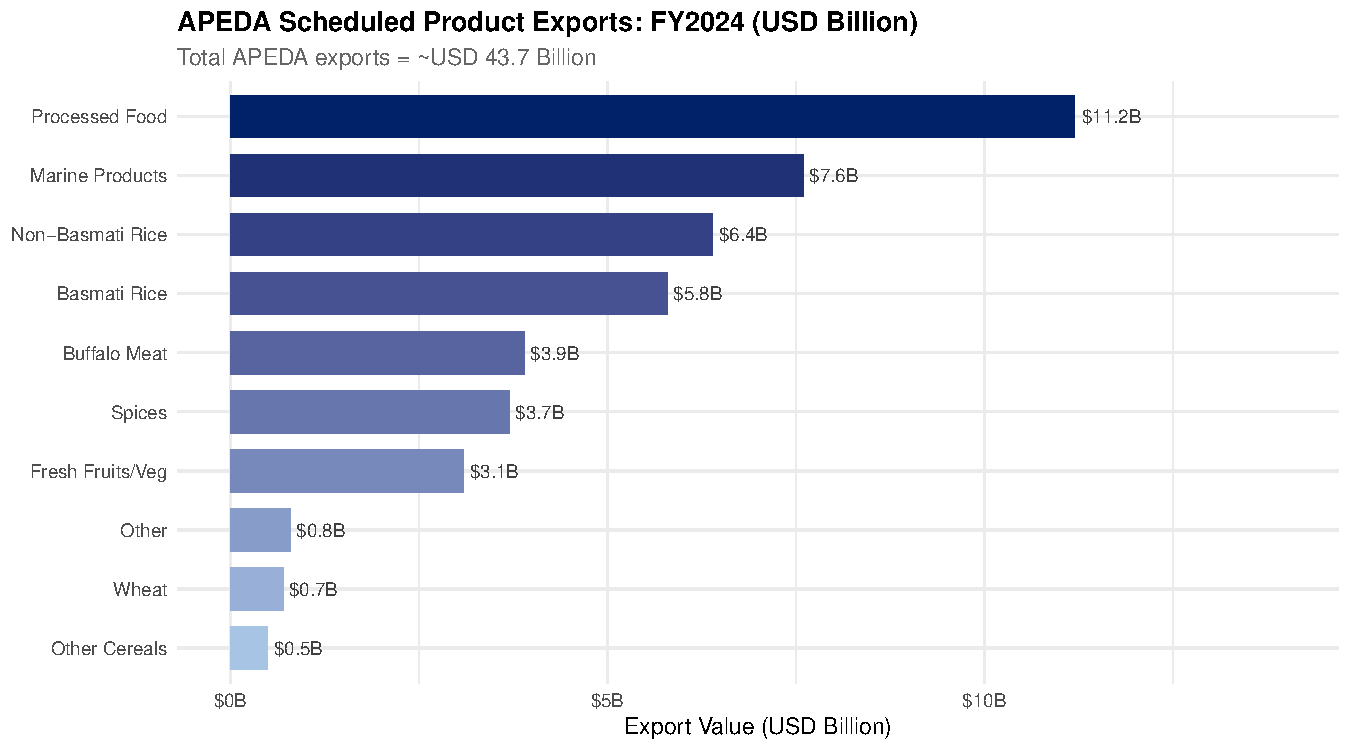
\includegraphics[keepaspectratio]{Lecture17_Export_Organizations_files/figure-beamer/fig-apeda-products-1.pdf}}

}

\caption{\label{fig-apeda-products}Processed food is the single largest
APEDA export category; marine products rank second. Rice (basmati +
non-basmati) together constitute \textasciitilde28\% of the basket.
Source: APEDA Annual Report 2023-24.}

\end{figure}%
\end{block}
\end{frame}

\begin{frame}
\begin{block}{APEDA's Key Functions in Practice}
\phantomsection\label{apedas-key-functions-in-practice}
\begin{columns}[T]
\begin{column}{0.5\linewidth}
\textbf{1. Financial Assistance (MDA Grants):}

\begin{itemize}
\tightlist
\item
  \textbf{Infrastructure:} pack houses, pre-cooling facilities, CA
  stores, vapour heat treatment (VHT) plants --- subsidy up to 50\% of
  cost (cap ₹50 lakh--₹3 crore)
\item
  \textbf{Quality labs:} NABL accreditation support; pesticide residue
  testing equipment
\item
  \textbf{Market promotion:} 75\% reimbursement of stall cost at
  international fairs
\end{itemize}

\textbf{2. Quality Standards:}

\begin{itemize}
\tightlist
\item
  Issues guidelines for pesticide residue management (grape, mango
  protocols)
\item
  Coordinates NABL-accredited testing laboratories for certifying
  shipments
\item
  Manages \textbf{Generic India brand} (Incredible India! branding at
  trade fairs)
\end{itemize}
\end{column}

\begin{column}{0.5\linewidth}
\textbf{4. Bilateral Market Access Protocols:}

Market access for perishables requires country-to-country pest risk
assessment (PRA). APEDA negotiates these protocols:

\begin{longtable}[]{@{}lll@{}}
\toprule\noalign{}
Protocol & Country & Product \\
\midrule\noalign{}
\endhead
VHT Protocol & \textbf{Japan} & Mango (Alphonso) \\
Cold Treatment & \textbf{South Korea} & Grapes \\
Systems Approach & \textbf{USA} & Mangoes \\
Residue Monitoring & \textbf{EU} & Grapes, pomegranate \\
\bottomrule\noalign{}
\end{longtable}

\textbf{The Japan mango success story:}\\
APEDA negotiated a \textbf{vapour heat treatment (VHT) protocol} with
Japan's Ministry of Agriculture (MAFF) in 2006. Indian mango exports to
Japan grew from near-zero to \textbf{\$50+ million} in FY2024.
\end{column}
\end{columns}

\note{\textbf{3. Market Intelligence:}

\begin{itemize}
\tightlist
\item
  APEDA's AgriXchange portal: real-time export statistics, market
  prices, tariff information for 50+ destinations
\item
  Issues market intelligence reports on key commodities and destinations
\item
  Organises buyer-seller meets (BSMs) in India and abroad
\item
  Publishes commodity-specific export guidelines and market reports
\end{itemize}}
\end{block}
\end{frame}

\begin{frame}
\begin{block}{Top 10 Destinations for India's Agricultural Exports}
\phantomsection\label{top-10-destinations-for-indias-agricultural-exports}
\begin{figure}

\centering{

\pandocbounded{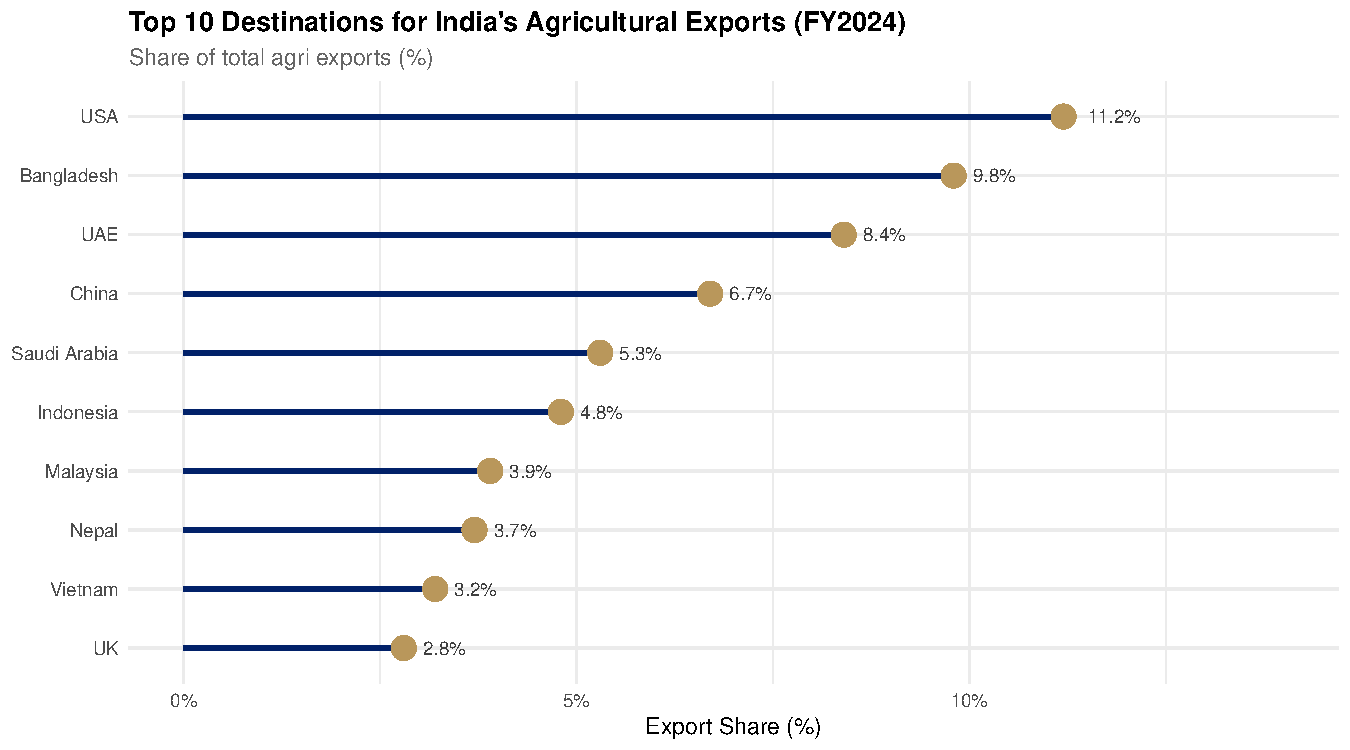
\includegraphics[keepaspectratio]{Lecture17_Export_Organizations_files/figure-beamer/fig-agri-destinations-1.pdf}}

}

\caption{\label{fig-agri-destinations}USA leads with 11.2\% share driven
by marine products and spices; Bangladesh and UAE are the next largest
markets for rice and meat exports. Source: APEDA Annual Report 2023-24.}

\end{figure}%
\end{block}
\end{frame}

\begin{frame}
\begin{block}{APEDA's Success Metrics: Selected Achievements}
\phantomsection\label{apedas-success-metrics-selected-achievements}
\begin{columns}[T]
\begin{column}{0.55\linewidth}
\textbf{Basmati Rice:}

\begin{itemize}
\tightlist
\item
  FY2010 export: \$1.5 billion\\
\item
  FY2024 export: \textbf{\$5.8 billion} (50+ destinations)
\item
  APEDA's GI application for Basmati at WTO (ongoing): protects brand
  value
\item
  APEDA basmati traceability: QR code on bags linking to farm, miller,
  testing report
\end{itemize}

\textbf{Organic Exports:}

\begin{itemize}
\tightlist
\item
  FY2024: \textbf{\$1.1 billion} (50+ countries)
\item
  India: 4th largest organic area globally (4.43 million ha, 4.5 million
  farmers)
\item
  APEDA manages NPOP (National Programme for Organic Production) ---
  certification, accreditation
\item
  USA (37\%) and EU (35\%) are top organic destinations
\end{itemize}

\textbf{Fresh Grapes (EU):}

\begin{itemize}
\tightlist
\item
  EU had threatened ban due to pesticide residues (2014 crisis)
\item
  APEDA's Grape Net portal: farmer-level residue monitoring of 1.5 lakh
  acres
\item
  Residue violations reduced from 180 (2013) to 9 (FY2024)
\item
  Grape exports: \textbf{\$260 million} FY2024; sustained EU market
  access
\end{itemize}
\end{column}

\begin{column}{0.45\linewidth}
\textbf{APEDA trade fair presence:}

\begin{longtable}[]{@{}lll@{}}
\toprule\noalign{}
Fair & Location & India Stall \\
\midrule\noalign{}
\endhead
Gulfood & Dubai, Feb & \textasciitilde400 exhibitors \\
SIAL & Paris, Oct & \textasciitilde150 exhibitors \\
Annapoorna & Mumbai & Domestic + buyers \\
FMI Show & Chicago & Marine, organic \\
WorldFood & Moscow & Basmati, spices \\
\bottomrule\noalign{}
\end{longtable}

APEDA's ``India Pavilion'' concept --- government-funded stall space
offered to SME exporters at subsidised rates. In FY2024, APEDA
facilitated participation of \textbf{3,200 exporters} across 47
international fairs.
\end{column}
\end{columns}
\end{block}
\end{frame}

\begin{frame}
\begin{block}{India Agricultural Exports: Long-run Trend}
\phantomsection\label{india-agricultural-exports-long-run-trend}
\begin{figure}

\centering{

\pandocbounded{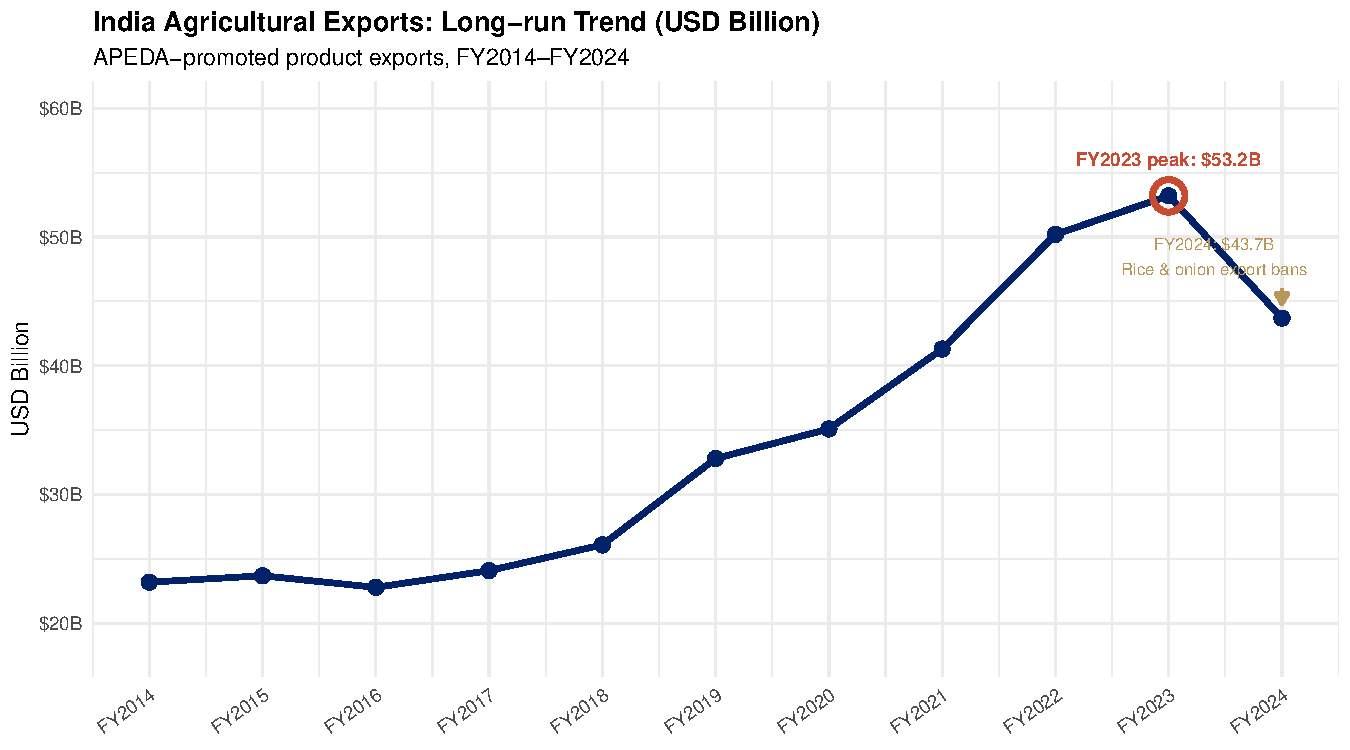
\includegraphics[keepaspectratio]{Lecture17_Export_Organizations_files/figure-beamer/fig-apeda-trend-1.pdf}}

}

\caption{\label{fig-apeda-trend}India's APEDA-promoted exports grew 2.3x
from FY2014 to the FY2023 peak of 53.2B USD, before declining to 43.7B
in FY2024 after non-basmati rice and onion export bans. Source: APEDA
Annual Report 2023-24.}

\end{figure}%
\end{block}
\end{frame}

\begin{frame}
\begin{block}{MPEDA: India's Seafood Export Authority}
\phantomsection\label{mpeda-indias-seafood-export-authority}
\begin{columns}[T]
\begin{column}{0.55\linewidth}
\textbf{MPEDA} --- Marine Products Export Development Authority

\begin{itemize}
\tightlist
\item
  Established under \textbf{MPEDA Act, 1972}
\item
  Ministry of Commerce and Industry
\item
  Headquarters: \textbf{Kochi, Kerala}; offices in all coastal states
\end{itemize}

\textbf{India's seafood exports (FY2024):}

\begin{itemize}
\tightlist
\item
  Total: \textbf{\$7.6 billion} (3.5 million MT)
\item
  India: \textbf{4th largest} seafood exporter globally (after China,
  Norway, Vietnam)
\item
  Shrimp: 66\% of export value
\item
  Top markets: USA (24\%), EU (22\%), China (14\%), Japan (8\%),
  Southeast Asia (7\%)
\end{itemize}

\textbf{Product mix:}

Frozen shrimp · Dried fish · Frozen fish (ribbonfish, pomfret) ·
Cephalopods (squid, cuttlefish, octopus) · Fresh/chilled fish · Seaweed
· Surimi

\textbf{Andhra Pradesh} contributes \textbf{70\% of India's shrimp
exports} --- the largest concentration of aquaculture in the world
outside China.
\end{column}

\begin{column}{0.45\linewidth}
\textbf{MPEDA's registration system:}

All marine product exporters must register with MPEDA. As of FY2024:

\begin{itemize}
\tightlist
\item
  Processing plants: \textbf{1,200+} (EU-approved: 350+)
\item
  Hatcheries: \textbf{2,800}
\item
  Aquaculture farmers linked: \textbf{\textasciitilde1.2 million}
\end{itemize}

\textbf{Traceability and CoC (Chain of Custody):}

MPEDA's CoC system tracks shrimp from farm pond to export container:

\begin{enumerate}
\tightlist
\item
  Farm registration (GPS-tagged)
\item
  Feed purchase records (antibiotic-free)
\item
  Harvest sampling (NRCP residue test)
\item
  Processing plant records
\item
  Container ID linked to farm batch
\end{enumerate}

This traceability is required for EU and USA market access --- buyers
can scan a QR code and trace any pack of Indian shrimp to the source
farm.
\end{column}
\end{columns}
\end{block}
\end{frame}

\begin{frame}
\begin{block}{MPEDA: Quality Systems and International Compliance}
\phantomsection\label{mpeda-quality-systems-and-international-compliance}
\begin{columns}[T]
\begin{column}{0.55\linewidth}
\textbf{National Residue Control Plan (NRCP):}

The EU requires all third-country seafood exporters to operate an NRCP
--- a systematic national programme testing for:

\begin{itemize}
\tightlist
\item
  Antibiotics (nitrofurans, chloramphenicol, tetracyclines)
\item
  Heavy metals (mercury, lead, cadmium)
\item
  Pesticide residues
\end{itemize}

MPEDA coordinates NRCP testing across states: - 18,000+ samples per year
- Tested at CIFT, EIC, and NABL labs - Annual audit by EU's DG-SANTE
(Health and Food Safety)

\textbf{Result:} EU has kept Indian seafood on its approved list
continuously since 2006 (minor suspension in 2002 was reversed after
MPEDA reforms).
\end{column}

\begin{column}{0.45\linewidth}
\textbf{USA FDA import alerts --- India's challenge:}

The USA FDA has issued import alerts on Indian shrimp over antibiotic
residues multiple times.

\textbf{2022 import alert:} 46 Indian processing plants placed under
increased surveillance; exports to USA dipped 8\% in FY2023.

\textbf{MPEDA's response:} - Mandatory antibiotic-free certification for
all USA-bound shrimp - MPEDA training for 50,000 Andhra farmers on
prohibited antibiotics - 3rd party testing at NABL labs (EIC, SGS)
before shipment

\textbf{Outcome:} USA-bound exports recovered to \$1.8B in FY2024.

SPS compliance is not a one-time event --- it requires continuous
investment in testing, farmer training, and government--industry
coordination.
\end{column}
\end{columns}
\end{block}
\end{frame}

\begin{frame}
\begin{block}{The Five Commodity Boards: Overview}
\phantomsection\label{the-five-commodity-boards-overview}
\begin{longtable}[]{@{}
  >{\raggedright\arraybackslash}p{(\linewidth - 10\tabcolsep) * \real{0.1667}}
  >{\raggedright\arraybackslash}p{(\linewidth - 10\tabcolsep) * \real{0.1667}}
  >{\raggedright\arraybackslash}p{(\linewidth - 10\tabcolsep) * \real{0.1667}}
  >{\raggedright\arraybackslash}p{(\linewidth - 10\tabcolsep) * \real{0.1667}}
  >{\raggedright\arraybackslash}p{(\linewidth - 10\tabcolsep) * \real{0.1667}}
  >{\raggedright\arraybackslash}p{(\linewidth - 10\tabcolsep) * \real{0.1667}}@{}}
\toprule\noalign{}
\begin{minipage}[b]{\linewidth}\raggedright
Board
\end{minipage} & \begin{minipage}[b]{\linewidth}\raggedright
Est.
\end{minipage} & \begin{minipage}[b]{\linewidth}\raggedright
HQ
\end{minipage} & \begin{minipage}[b]{\linewidth}\raggedright
Key Products
\end{minipage} & \begin{minipage}[b]{\linewidth}\raggedright
FY2024 Export
\end{minipage} & \begin{minipage}[b]{\linewidth}\raggedright
Top Markets
\end{minipage} \\
\midrule\noalign{}
\endhead
\textbf{Tea Board} & 1953 & Kolkata & CTC tea, orthodox, green &
\textasciitilde\$750M & Russia, UAE, UK \\
\textbf{Coffee Board} & 1942 & Bengaluru & Arabica, Robusta &
\textasciitilde\$1.2B & Italy, Germany, USA \\
\textbf{Rubber Board} & 1947 & Kottayam & NR, latex, crepe &
\textasciitilde\$250M & Germany, USA, Italy \\
\textbf{Spices Board} & 1987 & Kochi & Chilli, cumin, cardamom, pepper &
\textasciitilde\$3.7B & China, USA, Vietnam \\
\textbf{Tobacco Board} & 1976 & Guntur & FCV tobacco, cheroots &
\textasciitilde\$800M & Belgium, Germany, Russia \\
\bottomrule\noalign{}
\end{longtable}

All five boards perform similar functions: \textbf{research, quality
standards, market development, financial assistance, and export
promotion.} Each has a statutory role in the respective value chain ---
from regulating auctions (Tea, Tobacco) to issuing GI certificates
(Spices Board for Alleppey Green Cardamom).
\end{block}
\end{frame}

\begin{frame}
\begin{block}{Tea Board of India}
\phantomsection\label{tea-board-of-india}
\begin{columns}[T]
\begin{column}{0.55\linewidth}
\textbf{India's tea sector:}

\begin{itemize}
\tightlist
\item
  \textbf{2nd largest producer globally} (after China): 1.35 billion
  kg/year (FY2024)
\item
  Domestic consumption: \textasciitilde1.1 billion kg (India is its own
  largest consumer)
\item
  Exports: \textbf{200--250 million kg (\textasciitilde\$750--800
  million)}
\end{itemize}

\textbf{Tea Board functions:}

\begin{itemize}
\tightlist
\item
  Regulates tea auctions: \textbf{Kolkata, Guwahati, Coimbatore, Cochin}
  auction centres
\item
  Tea Research Association (Tocklai, Assam): oldest tropical crop
  research station in the world (est. 1911)
\item
  Issues \textbf{Tea Certificate} for all shipments
\item
  Darjeeling GI: \textbf{world's first GI-tagged tea} (EU recognition
  1995, India 2004). 87 registered gardens. \textasciitilde7 million
  kg/year.
\end{itemize}

\textbf{Top export markets:} Russia (20\%), UAE (18\%), UK (12\%), USA
(7\%), Germany (5\%)
\end{column}

\begin{column}{0.45\linewidth}
\textbf{Challenges facing Indian tea:}

\begin{enumerate}
\tightlist
\item
  \textbf{Competition:} Kenya (low-cost CTC), China (premium
  green/white), Sri Lanka (strong Ceylon brand)
\item
  \textbf{Price stagnation:} Assam CTC auction prices have grown only
  4\% annually since 2015 despite input cost inflation
\item
  \textbf{Climate risk:} North Bengal tea gardens face erratic monsoon;
  2023 drought cut Darjeeling first-flush yield by 30\%
\item
  \textbf{Small-tea growers:} 35\% of tea production from 200,000+ small
  growers (\textless{} 10 ha) --- difficult to comply with Rainforest
  Alliance/UTZ standards required by European retail chains
\end{enumerate}

\textbf{Tea Board response:} Grameen Krishi Mitra (GKM) extension
workers linking small growers to certification. Target: 50\% certified
by 2028.
\end{column}
\end{columns}
\end{block}
\end{frame}

\begin{frame}
\begin{block}{Coffee Board and Spices Board}
\phantomsection\label{coffee-board-and-spices-board}
\begin{columns}[T]
\begin{column}{0.5\linewidth}
\textbf{Coffee Board of India (est. 1942, Bengaluru):}

\begin{itemize}
\tightlist
\item
  India: \textbf{3rd largest Arabica producer in Asia}
\item
  Production: \textasciitilde350,000 MT/year
\item
  Exports: \textbf{\$1.2 billion (FY2024)} --- record high; 15\% growth
  over FY2023
\item
  {Arabica}: Coorg, Chikmagalur (Bababudangiri GI); shade-grown, organic
  premium
\item
  {Robusta}: Wayanad, Hassan; used in espresso blends globally
\item
  Top markets: Italy (30\%), Germany (18\%), Belgium (12\%), USA (9\%)
\item
  CCRI (Central Coffee Research Institute, Chikmagalur):
  disease-resistant variety development
\item
  Specialty coffee promotion: India now at World Barista Championship;
  ``Indian single origin'' brand growing
\end{itemize}

Coffee Board's \textbf{Café Coffee Day} predecessor was a Board
initiative. Domestic coffee consumption now growing 7\% annually ---
youngest coffee drinking demographic globally.
\end{column}

\begin{column}{0.5\linewidth}
\textbf{Spices Board of India (est. 1987, Kochi):}

\begin{itemize}
\tightlist
\item
  India: \textbf{world's largest spice exporter by value}
\item
  109 varieties; 8 million MT production; \textbf{4.5 million MT
  exports}
\item
  \textbf{\$3.7 billion (FY2024)} --- 5-year CAGR of 12\%
\end{itemize}

\textbf{Top export items (FY2024):}

\begin{longtable}[]{@{}ll@{}}
\toprule\noalign{}
Spice & Value \\
\midrule\noalign{}
\endhead
Chilli & \$1.1B \\
Spice Oils \& Oleoresins & \$800M \\
Cumin & \$720M \\
Turmeric & \$200M \\
Cardamom & \$150M \\
Pepper & \$140M \\
\bottomrule\noalign{}
\end{longtable}

\textbf{GI products:} Alleppey Green Cardamom, Malabar Black Pepper,
Guntur Sannam Chilli, Coorg Orange Cardamom. Premium over non-GI:
\textbf{20--40\%} in EU market.

\textbf{SPS challenge:} EU raised MRL concerns on Indian chilli (Sudan
Red dye, aflatoxin). Spices Board's GAP training programme covers
500,000 chilli farmers in Andhra Pradesh.
\end{column}
\end{columns}
\end{block}
\end{frame}

\begin{frame}
\begin{block}{Export Inspection Council (EIC)}
\phantomsection\label{export-inspection-council-eic}
\begin{columns}[T]
\begin{column}{0.55\linewidth}
\textbf{EIC} --- statutory body under the \textbf{Export (Quality
Control and Inspection) Act, 1963}

\begin{itemize}
\tightlist
\item
  Ministry of Commerce and Industry; HQ New Delhi
\item
  Purpose: independent certification that Indian exports meet quality
  standards acceptable to importing countries
\end{itemize}

\textbf{Structure:}

\begin{itemize}
\tightlist
\item
  \textbf{5 regional EIOs} (Export Inspection Offices): Mumbai, Chennai,
  Kochi, Kolkata, Delhi
\item
  \textbf{40+ sub-offices} in export-intensive centres (Vizag, Surat,
  Amritsar, Ludhiana)
\item
  Accredited by \textbf{EU's DG-SANTE, USFDA, Japan MHLW, Korean MFDS}
\end{itemize}

\textbf{Mandatory certification products:}

Fish and fishery products · Meat and meat products · Poultry products ·
Dairy products · Egg products · Honey · Organic products · Castor oil ·
Processed food (for EU, Japan, USA)
\end{column}

\begin{column}{0.45\linewidth}
\textbf{What EIC does per shipment:}

\begin{enumerate}
\tightlist
\item
  Document verification (invoice, packing list, test reports)
\item
  Physical inspection: random sampling from lot
\item
  Lab analysis: microbiological, chemical, pesticide, heavy metals
\item
  Issuance of \textbf{Health Certificate} (format accepted by
  destination country)
\item
  Post-shipment surveillance: tracks rejection reports from destination
\end{enumerate}

\textbf{EIC performance (FY2024):}

\begin{itemize}
\tightlist
\item
  Certificates issued: \textbf{1.8 lakh}
\item
  Value covered: \textbf{₹1.1 lakh crore}
\item
  Rejection rate (border rejections at EU/USA): \textbf{0.4\%} (one of
  the lowest among major exporters)
\item
  Turnaround time: \textbf{2--3 working days} for most certificates
\end{itemize}

An \textbf{FSSAI-EIC joint protocol} (2022) has harmonised testing
requirements so exporters need not test separately for domestic FSSAI
and export EIC compliance.
\end{column}
\end{columns}
\end{block}
\end{frame}

\begin{frame}
\begin{block}{NAFED: Price Stabilisation and Export Implications}
\phantomsection\label{nafed-price-stabilisation-and-export-implications}
\begin{columns}[T]
\begin{column}{0.55\linewidth}
\textbf{NAFED} --- National Agricultural Cooperative Marketing
Federation of India

\begin{itemize}
\tightlist
\item
  Established 1958; cooperative society under Multi-State Cooperative
  Societies Act
\item
  Functions: \textbf{Price Support Scheme (PSS) procurement}, buffer
  stock management, retail distribution
\end{itemize}

\textbf{PSS and its export connection:}

When prices of oilseeds (mustard, groundnut, soybean) and pulses fall
below MSP: - Government activates PSS; NAFED procures from farmers at
MSP - NAFED accumulates buffer stocks of oilseeds/pulses - Stocks are
sold through NAFED retail, e-commerce, and open market sales when prices
rise - Procurement \textbf{reduces export availability} (absorbs
domestic surplus before it can be exported); but \textbf{stabilises farm
incomes}

In kharif 2023: NAFED procured \textbf{38 lakh MT of tur dal} at MSP
(₹6,600/quintal) from Karnataka, Maharashtra, Madhya Pradesh. This stock
was later released to control prices --- but reduced the quantity
available for the export market in FY2024.
\end{column}

\begin{column}{0.45\linewidth}
\textbf{The NAFED export dilemma:}

NAFED is \textbf{not primarily an export organization} --- it is a price
stabilisation agency. But its procurement and buffer management
decisions directly affect India's agri export supply.

\textbf{Tension:} When NAFED holds large tur dal stocks, export prices
are firm because domestic supply is constrained. When NAFED releases
stocks, domestic prices fall → farmer incomes hurt, but consumers
benefit.

\textbf{FPO linkage:}

NAFED's eMandis portal now links FPOs to government procurement at MSP
and to private buyers. 1,200 FPOs linked as of FY2024, aggregating
procurement from 2.5 million farmers.

\textbf{AAPL (NAFED's retail arm):} sells agri commodities B2C through
1,200+ stores, Amazon/Flipkart --- brand building for Indian agri.
\end{column}
\end{columns}
\end{block}
\end{frame}

\begin{frame}
\begin{block}{Farmer Producer Organizations as Export Units}
\phantomsection\label{farmer-producer-organizations-as-export-units}
\begin{columns}[T]
\begin{column}{0.55\linewidth}
\textbf{The small-farm problem:}

India's average farm size: \textbf{1.08 hectares} (Agriculture Census
2015--16).\\
Average EU/USA buyer minimum order: \textbf{20 MT per lot.}

No individual smallholder can meet buyer requirements for: - Consistent
volume - Uniform quality and grading - Traceable production records -
Third-party certification costs (organic, GlobalGAP)

\textbf{FPOs as aggregators:}

An FPO with 500 members × 1 ha each = 500 ha aggregate. Can produce
300--500 MT of a single crop --- meeting buyer minimums.
\end{column}

\begin{column}{0.45\linewidth}
\textbf{Successful FPO export examples:}

\textbf{Mahagrapes (Maharashtra):}\\
Cooperative of 46 grape-growing cooperatives, \textasciitilde25,000
farmers.\\
Exports EU-compliant grapes to Netherlands, Germany, UK.\\
FY2024 exports: \textasciitilde8,000 MT (\textasciitilde\$40M).\\
Uses APEDA-funded pack houses and cold chain in Nashik.

\textbf{Sahyadri Farms (Nashik):}\\
12,000 farmer members; India's largest single FPO.\\
GlobalGAP certified; supplies Tesco UK, Carrefour.\\
Own cold chain, pack house, CA storage.

\textbf{NDDB dairy cooperatives:}\\
Amul (GCMMF): 3.6 million farmer members; dairy exports to 50+ countries
\textasciitilde\$500M.

\textbf{APEDA's FPO Connect:} 1,200+ FPOs registered, linked to APEDA's
buyer database and MDA grant system. FPOs can now access MDA grants
directly --- not just through large exporters.
\end{column}
\end{columns}
\end{block}
\end{frame}

\begin{frame}
\begin{block}{Government Schemes Supporting Agri Export Organizations}
\phantomsection\label{government-schemes-supporting-agri-export-organizations}
\begin{columns}[T]
\begin{column}{0.5\linewidth}
\textbf{PM FME (Formalisation of Micro Food Enterprises) Scheme:} -
₹10,000 crore over 5 years (2020--25) - Credit-linked subsidy (35\%) for
micro-enterprises upgrading to FSSAI standards - ODOP (One District One
Product) focus products receive priority - 2 lakh+ enterprises
formalized by FY2024 → many now eligible for export

\textbf{NABARD's Agri Infrastructure Fund (AIF):} - ₹1 lakh crore; 3\%
interest subvention - Pack houses, cold stores, CA chambers, primary
processing centres - Linked to FPO and cooperative projects --- directly
supports export infrastructure

\textbf{SFAC (Small Farmers Agribusiness Consortium):} - FPO promotion,
equity grant support - Connects FPOs to APEDA/MPEDA registered exporters
- Pilot: 100 agri export FPOs linked directly to 3 commodity board
markets
\end{column}

\begin{column}{0.5\linewidth}
\textbf{APEDA-NHB Horticulture Export Collaboration:}

NHB (National Horticulture Board) funds pack houses; APEDA funds market
promotion. Joint program in: - Banana (Jalgaon, Maharashtra → Middle
East) - Guava (Allahabad, UP → UK diaspora market) - Litchi
(Muzaffarpur, Bihar → EU, West Asia)

\textbf{Districts as Export Hubs (DEH) --- FTP 2023--28:}

Commerce Ministry has identified \textbf{100+ districts} with specific
``champion products.''

Examples: - Kalaburagi (Karnataka): Tur dal - Nashik (Maharashtra):
Grapes, onions - Tirupur (Tamil Nadu): Knitwear + agri - Coorg
(Karnataka): Coffee, pepper - Guntur (Andhra Pradesh): Chilli, turmeric

District Collectors coordinate between farmers, FPOs, exporters, and
commodity boards. Target: every DEH district to double export value in 5
years.
\end{column}
\end{columns}
\end{block}
\end{frame}

\begin{frame}
\begin{block}{India's 2030 Agricultural Export Ambition}
\phantomsection\label{indias-2030-agricultural-export-ambition}
\begin{columns}[T]
\begin{column}{0.55\linewidth}
\textbf{APEDA's target: \$60 billion by 2030}\\
(from \$43.7B in FY2024; required CAGR \textasciitilde5.4\%)

\textbf{MPEDA's target: \$12 billion in seafood}\\
(from \$7.6B; focus on value-added and ready-to-eat)

\textbf{Commodity Board targets:} - Spices Board: \$5B (from \$3.7B) -
Coffee Board: \$2B (from \$1.2B) - Tea Board: \$1.5B (from \$750M)

\textbf{Overall national agri-food export target (FTP 2023--28): \$100
billion by 2030}

\textbf{Strategy pillars:} 1. Diversify beyond rice dominance 2. Open
new markets: Africa, Southeast Asia, South Korea 3. Value addition:
processed, organic, functional foods 4. Invest in cold chain: PM
GatiShakti nodes 5. Leverage GI brand premiums 6. FTA market access:
India-UAE CEPA live; India-UK FTA being negotiated
\end{column}

\begin{column}{0.45\linewidth}
\textbf{Key Takeaways:}

\begin{enumerate}
\tightlist
\item
  \textbf{APEDA} is the backbone of India's agri export promotion ---
  covers 60\% of the export basket
\item
  \textbf{MPEDA} manages India's \$7.6B seafood export with rigorous
  quality systems essential for EU/USA access
\item
  \textbf{Commodity Boards} are sector-specific engines --- Spices
  Board's \$3.7B is remarkable for a relatively small value chain
\item
  \textbf{EIC} provides the third-party quality assurance without which
  EU/USA market access is impossible
\item
  \textbf{FPOs} are solving the small-farm aggregation problem ---
  Mahagrapes, Sahyadri, Amul show it is achievable at scale
\item
  \textbf{District-level implementation} through DEH is the newest
  institutional innovation --- connecting national targets to local
  value chains
\end{enumerate}
\end{column}
\end{columns}
\end{block}
\end{frame}

\begin{frame}
\begin{block}{Next Lecture}
\phantomsection\label{next-lecture}
\textbf{Lecture 18 --- India's Agricultural Trade and Foreign Trade
Policy}\\
\emph{August 22, 2026 --- FINAL LECTURE}

\begin{itemize}
\tightlist
\item
  Course synthesis: from comparative advantage to India's \$43.7 billion
  agri export reality
\item
  India's trade performance: FY2024 big picture and 10-year trends
\item
  Export composition, import profile, and the value-addition opportunity
\item
  Foreign Trade Policy 2023--28: vision, themes, and agricultural
  provisions
\item
  Millets, GIs, and organic exports as strategic niches
\item
  Challenges India must overcome and opportunities ahead
\item
  The farmer welfare vs export competitiveness dilemma
\item
  Course synthesis: what 18 weeks has taught us
\item
  India's Agricultural Export Vision 2030
\end{itemize}

\textbf{Final lecture preparation:} Review all lecture notes from
Lectures 1--17. Bring questions --- we will have a 15-minute open Q\&A
on examination topics at the end of Lecture 18.
\end{block}
\end{frame}

\begin{frame}{Appendix}
\phantomsection\label{appendix}
\begin{block}{Additional Resources}
\phantomsection\label{additional-resources}
\begin{columns}[T]
\begin{column}{0.5\linewidth}
\textbf{Further Reading}

\begin{itemize}
\tightlist
\item
  Lecture notes and APEDA/WTO official documents
\item
  APEDA Annual Report 2023-24
\item
  RBI/DGCI\&S/APEDA databases for latest data
\end{itemize}
\end{column}

\begin{column}{0.5\linewidth}
\textbf{Key Data Sources}

\begin{itemize}
\tightlist
\item
  DGCI\&S: India's merchandise trade
\item
  RBI: Balance of payments data\\
\item
  APEDA: Agricultural export statistics
\item
  WTO: Tariff and trade databases
\end{itemize}
\end{column}
\end{columns}
\end{block}
\end{frame}




\end{document}
